\subsection{Descri\c c\~ao do Problema} \label{subsec:descricao}

A descrição do problema é fundamental para obter uma compreensão mais precisa do que está sendo abordado neste trabalho. É por meio dessa descrição que as variáveis-chave são expostas e o objetivo da previsão é estabelecido de forma clara. Sem um plano estruturado para determinar o que deve ser previsto, torna-se difícil justificar o uso de modelos de previsão de dados. Portanto, é essencial estabelecer um propósito claro e definir as metas da previsão antes de aplicar os modelos adequados.

\begin{itemize}
	\item Bombas de sucção (B1, B2 e B3) – valor máximo da frequência 60 Hz
	
	\item Nível do Reservatório (Câmara 1) LT01 $ (m^3) $ - \textbf{PREVER}
	
	\item Vazão de entrada (FT01) $ (m^3/h) $
	
	\item Vazão de gravidade (FT02) $ (m^3/h) $
	
	\item Vazão de recalque (FT03) $ (m^3/h) $
	
	\item Pressão de Sucção (PT01SU) (mca)
	
	\item Pressão de Recalque (PT02RBAL) (mca)
\end{itemize}

A pesquisa fará uso da variável LT01, que representa o nível do reservatório e desempenha um papel de extrema importância, como evidenciado pelas Figuras \ref{fig:dados-todos} e \ref{fig:2020-a-frente}. Essas figuras retratam as anomalias ocorridas durante o período em que a capital paranaense foi afetada pela escassez de chuvas, resultando na redução do nível dos reservatórios e na implementação de rodízios periódicos, conforme discutido na subseção \ref{subsubsec:motivacao}. Assim, tais observações permitem uma compreensão mais aprofundada das perspectivas futuras.

\subsection{Procedimentos Metodol{\'o}gicos} \label{subsec:metod}

Com o intuito de realizar previsões e fazer comparações entre os modelos obtidos na revisão sistemática, será adotado um processo metodológico bem definido. Tal processo está detalhado na subseção \ref{subsubsec:etp} desta seção, onde foram estabelecidas as etapas a serem seguidas. Isso inclui a definição do que será previsto, bem como a seleção dos métodos a serem utilizados na Análise Exploratória de Dados (EDA).
   

\subsubsection{Etapas da Pesquisa}\label{subsubsec:etp}

%A pesquisa foi conduzida seguindo as etapas delineadas:
%
%\begin{figure}[!htpb]
%	\centering
%	\caption{Mapa das Etapas}
%	\label{fig:etapas}
%	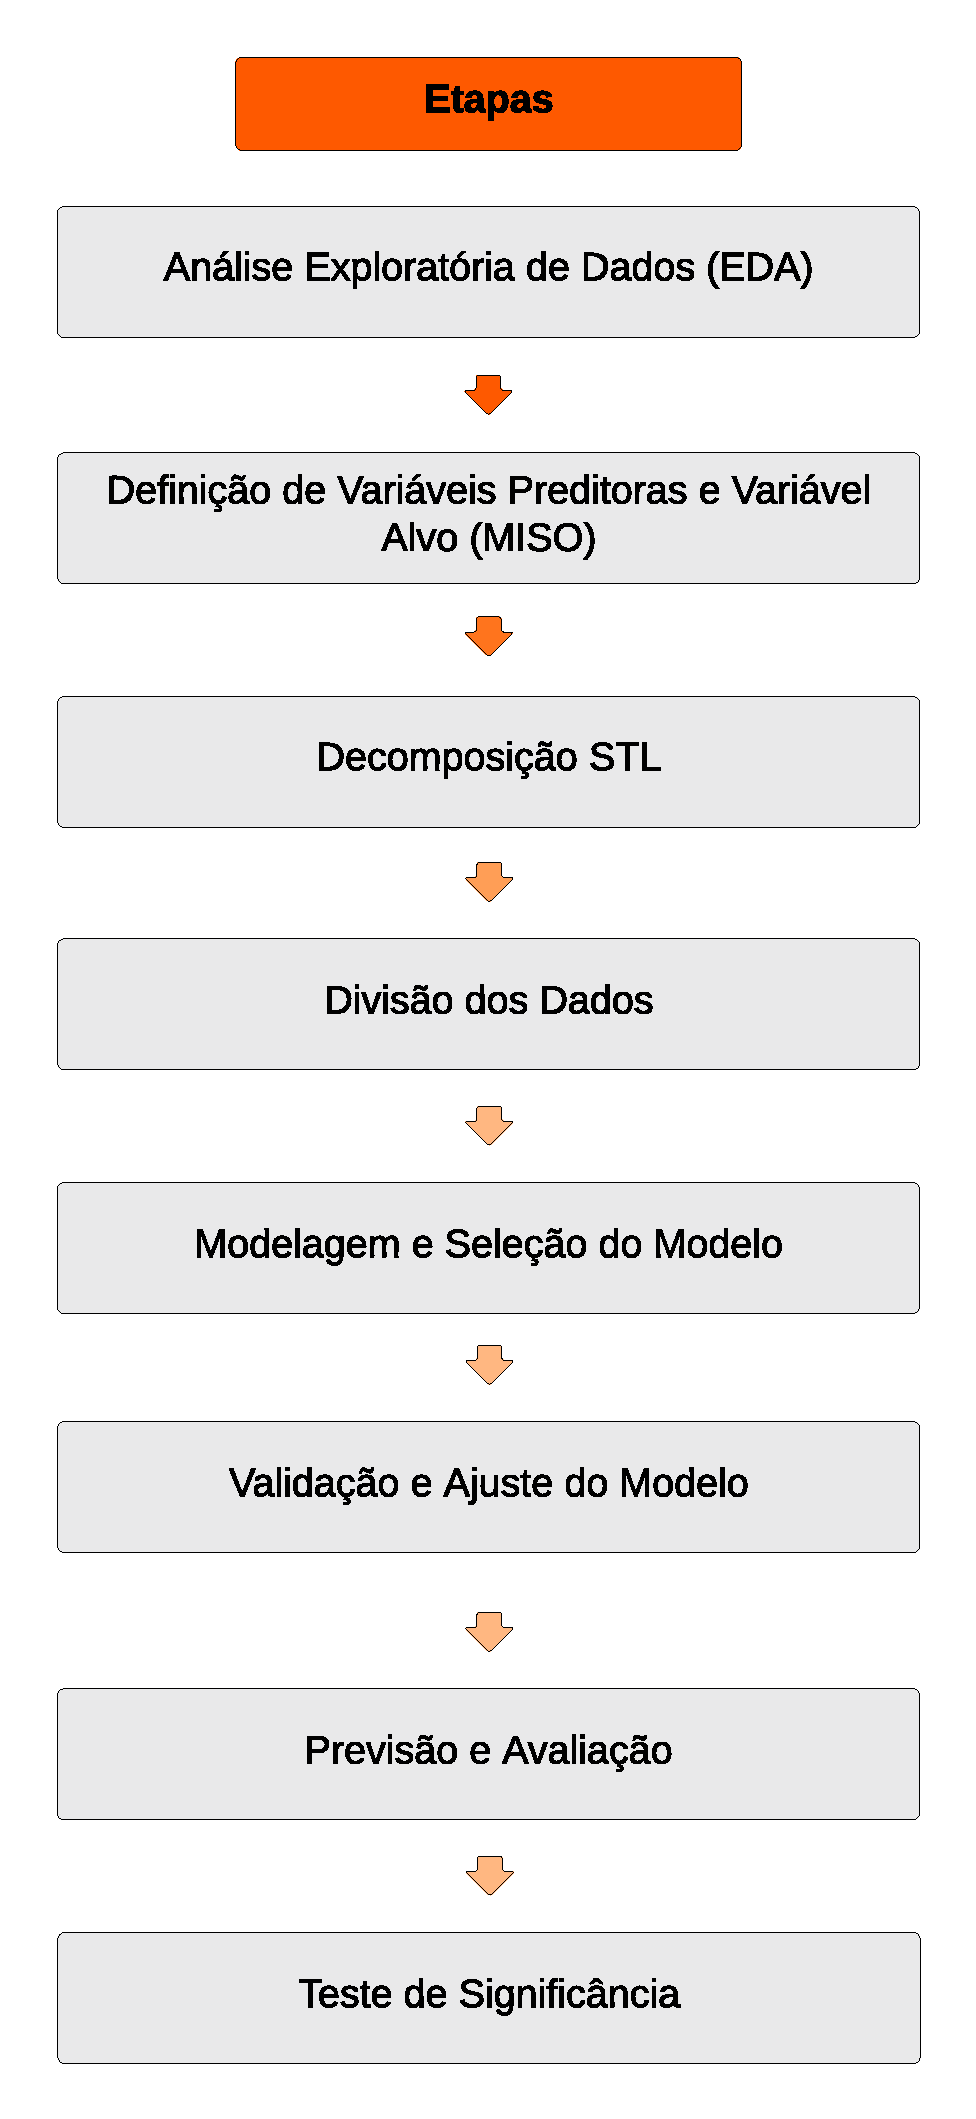
\includegraphics[width=1\linewidth]{Introducao/Figuras/Etapas}
%	
%	\fonte{De autoria própria}
%\end{figure}

\begin{enumerate}[start=1, label={\textbf{Etapa} \arabic*}]
	
	\item \label{etp:1} \textbf{Análise Exploratória de Dados (EDA)}: Nesta etapa inicial, compreende-se abrangentemente as características dos dados. As tarefas envolvem a identificação de valores ausentes, a observação de padrões temporais e a detecção de anomalias. Gráficos de linha são comuns para visualizar a convergência dos dados e desvios potenciais \cite{Rostam2021108249}.
	
	\item \label{etp:2} \textbf{Definição de Variáveis Preditoras e Variável Alvo (MISO)}: Na segunda etapa, as variáveis preditoras e a variável alvo para a previsão de Múltiplas Entradas e Uma Saída (MISO) são selecionadas. Diferentes modelos, podem incorporar variáveis exógenas na modelagem. Essas variáveis adicionais aprimoram as capacidade de previsão do modelo, especialmente quando o horizonte de previsão se estende além dos dados históricos \cite{PAWLOWSKI202298}. 
	
	\item \label{etp:3} \textbf{Decomposição STL}: O método de decomposição STL (do inglês \textit{Seasonal and Trend Decomposition Using Loess}) separa uma série temporal em três componentes: sazonalidade, tendência e resíduo. Essa decomposição permite uma analisa separada das diferentes influências presentes nos dados. A componente sazonal representa variações periódicas e repetitivas, a componente de tendência indica a direção geral dos dados ao longo do tempo, e a componente de resíduo captura variações não explicadas pelas componentes anteriores \cite{DEOLIVEIRA2018776}.
	
	\item \label{etp:4} \textbf{Divisão dos Dados}: É prática comum dividir o conjunto de dados em conjuntos de treinamento, validação e teste para avaliar o desempenho do modelo. Essa divisão permite uma análise abrangente e objetiva das habilidades de generalização dos modelos, evitando problemas de ajuste excessivo ou insuficiente. A proporção de alocação pode variar, mas uma abordagem comum é alocar 70\% para treinamento e validação, e os 30\% restantes para o conjunto de testes. A porção de treinamento e validação pode ser subdividida em 80\% para treinamento e 20\% para validação \cite{Tao2020}.
	
	\item \label{etp:5} \textbf{Modelagem e Seleção do Modelo}: Nesta etapa, diversos modelos são construídos e avaliados. Alguns modelos comumente usados para previsão de séries temporais incluem ARX (do inglês \textit{Auto-Regressive with Exogenous Inputs}), AR (do inglês \textit{Auto-Regressive}), MA (do inglês \textit{Moving Average}), ARIMA, SARIMA (do inglês \textit{Seasonal Auto-Regressive Integrated Moving Averages}), SARIMAX (ARIMA Sazonal com variáveis exógenas) e modelos de aprendizado de máquina como RNN, LSTM (do inglês \textit{Long Short-Term Memory}), GRU (do inglês \textit{Gated Recurrent Unit}), Transformer (Transformador), DTR (do inglês \textit{Decision tree regressor}), LR (do inglês \textit{Linear Regression}), XGBoost (do inglês \textit{eXtreme Gradient Boosting}), Light GBM (do inglês \textit{Light Gradient Boosting Machine}) além do Prophet. A escolha do modelo final baseia-se em critérios como desempenho na validação, simplicidade do modelo e interpretabilidade dos resultados.
	
	\item \label{etp:6} \textbf{Validação e Ajuste do Modelo}: Após a construção do modelo, é importante avaliar seu desempenho usando dados de validação. Métricas de avaliação como Erro Médio Absoluto (MAE), Erro Médio Percentual Absoluto Simétrico (sMAPE) e Raiz do Erro Médio Quadrático Relativo (RRMSE) podem ser usadas para comparar e selecionar o melhor modelo. Além disso, técnicas de ajuste como otimização de hiperparâmetros e refinamento do modelo usando dados de treinamento e validação combinados podem melhorar o desempenho do modelo selecionado.
	
	\item \label{etp:7} \textbf{Previsão e Avaliação}: Com o modelo final ajustado, é possível fazer previsões para o conjunto de testes, que representa dados futuros não observados. Essas previsões são comparadas com os valores reais correspondentes para avaliar a qualidade e precisão do modelo. Métricas de desempenho mencionadas anteriormente (MAE, RRMSE, sMAPE) podem quantificar a precisão do modelo e compará-lo com outros modelos ou abordagens.
	
	\item \label{etp:8} \textbf{Teste de Significância}: Aplicar os modelos de previsão e fazer comparativo baseado em testes de significância estatística (\textit{Friedman e Nemenjy})

	
\end{enumerate}

Cada uma dessas etapas desempenha um papel crucial na pesquisa e no processo de modelagem de séries temporais, contribuindo para a compreensão dos dados, construção e validação dos modelos, além de previsões precisas.




    